\begin{document}
\maketitle
%\chapter{Backoff Grammar}

\section{Backoff Grammar}

Multi-category grammars can better represent complex structure and reordering useful in machine translation, but their power is limited by the sparsity of the training data.  Complex structures with limited representation in the grammar may not exist with sufficient contexts in the training data to be used to their fullest extent.  This is likely to cause problems when translating structurally divergent language pairs.

This portion of the project seeks to design a backoff grammar which can build on a multi-category grammar such as the one induced by the Pitman-Yor process described elsewhere in these proceedings.  The backoff grammar adds the flexibility of a single category grammar without sacrificing reordering.

In the Motivation section, the reason for designing such a grammar is explored in more detail.  In the Naive Backoff section is explained the original implementation of the backoff grammar, and in the Hierarchical Backoff section, the last tested iteration of the grammar is explained.  Results of both grammars on the BTEC corpus versus a single-category Hiero baseline are explained in the Results and Analysis section.  Finally, we will conclude with this part's role in the larger workshop project as well as describe possible future work in the Conclusions section.

\subsection{Naive Backoff}

As was previously mentioned, given the sparsity of the training data, no phrase will have all of its linguistically possible contexts accounted for in the grammar.  As an example, consider the production in (\ref{eq:whenwill}):

\begin{equation}\label{eq:whenwill}
X \rightarrow \text{when will }Y\text{ be }Z
\end{equation}

In English, this is a useful construction, and it is made more useful in translating Chinese, where it necessitates reordering to derive the most accurate translation.  However, this is only possible so long as the necessary phrases exist in categories Y and Z.  In the example thus far given, the English sentence ``when will they be ready" was possible with the rest of the grammar: ``they" existed as a possible production of Y, and ``ready" as a possible production of Z.  Some phrases, however, may not exist, despite the fact that they might well produce a more appropriate translation.  Suppose instead of ``they", one wanted to produce ``the pancakes" from Y, to create the valid sentence ``when will the pancakes be ready".  If Y does not have such a production, the derivation must be broken down into smaller chunks combined with glue rules, which may not have the reordering power of (\ref{eq:whenwill}).

This intuition can be applied to other instances, which will undoubtedly occur due to sparsity.  An induced grammar may cover many useful constructions, but in order for those constructions to be put to best use in a SCFG derivation, non-terminals should not be restricted to only those in the pre-existing induced grammar.  The most useful backoff grammar for translation would allow a rule to produce any other category (as is the case in a single category Hiero grammar), but prefer those constructions made most likely by the training data.  

In this formulation of the backoff grammar, additional rules were produced based on the induced multi-category grammar.  The set of non-terminals $T$ was doubled, such that for each non-terminal $X_k \in T$, a corresponding nonterminal $X-backoff_k$ was produced.  Each rule in the grammar was rewritten, replacing each $X_k$ on the RHS of the production with $X-backoff_k$.  Backoff rules were added for each $X-backoff_k$ with a possible RHS of any of the original non-terminals.  Backoff rules were assigned the feature BackoffRule, assigned 0 if $X-backoff_k$ had the RHS $X_k$ and 1 if $X-backoff_k$ had the RHS $X_j$ where $j \not = k$.

\begin{figure}
\label{fig:naivebo}
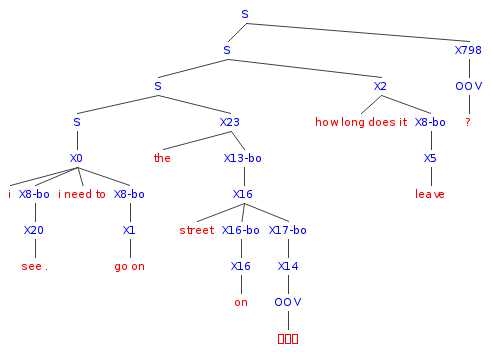
\includegraphics{naivebackoff.jpg}
\caption{A sample derivation using a multi-category grammar augmented with the naive version of the backoff grammar.
\end{figure}

Figure (\ref{fig:naivebo}) shows an example tree derived from an induced grammar which shows the behaviour of the backoff rules in a derivation.  Notice that X8-bo, replacing X8 in the original X0 production, produced an X20 and an X1 in this derivation, while X16-bo produced an X16 as expected.

This approach allowed derivations to utilize complex constructions like that in (\ref{eq:whenwill}), while still smoothing the output to allow alternate derivations of subconstituents.  The multi-category grammar can behave like a single-category grammar when it is more useful, with a penalty.

\subsection{Hierarchical Backoff}

The next iteration of the backoff grammar built on the naive backoff grammar, encoding a hierarchy of backoff rules.  The naive formulation of the grammar did not distinguish between the other categories except by the presence of other features.  Ideally, a backoff grammar would preferentially allow similar non-terminals to backoff to the same backoff category.

The hierarchical backoff process was another augmentation of the grammar, this time increasing the rules by creating sets of rules at different levels of the hierarchy.  A strict rule hierarchy, making certain non-terminals strictly more general than a set of other non-terminals, was not absolutely necessary.  Instead, this backoff process built the hierarchy based on the pre-existing grammar induction process, and determined category similarity based on the frequency of category assignment to phrases in the training data.

This rough hierarchy came from inducing some set $G$ of multi-category grammars, varying the level of granularity to $<x_1, x_2, \dots, x_n>$ where $n=|G|$.  A complete grammar consisted of the complete rulesets from each grammar in $G$, augmented with backoff rules.

For every grammar with number of categories $x_i | 1 \leq i < n$, a set of rules was added from each non-terminal $t_i$ in the $X_i$ grammar to each non-terminal $t_{i+1}$ in the $X_{i+1}$ grammar.  These rules were each assigned the BackoffRule feature, with feature weight as in (\ref{eq:ftrwgt}), based on the frequency of phrases $p$ which were assigned both categories.

\begin{equation}
\label{eq:ftrwgt}
BR = \log_2{P(t_{i+1} | t_i) \\
P(t_{i+1} | t_i) = \frac{count( \{p\text{ assigned category }t_i\} \cap \{p\text{ assigned category }t_{i+1}\} )}{count( \{p \text{ assigned category }t_i)} 
\end{equation}

The addition of these rules allowed backoff categories to be preferentially chosen which bore similarity to the category originally specified by the induced rule.

Though this hierarchy building process clearly does not create a true hierarchy, it also does not produce several unrelated levels of granularity.  As seen in (\ref{fig:entropy}), rougher categories bore a strong relation to several of the finer categories.

\begin{figure}
\label{fig:entropy}
\caption{Cross-entropy for the PYP-induced grammars.}

\includegraphics{hier-backoff.images/15-10.jpg}
\includegraphics{hier-backoff.images/30-105.jpg}
\end{figure}

\subsection{Results}

The backoff grammars were tested on BTEC and Urdu-English, using BLEU.  The naive backoff grammar did not have a strong effect on the results, causing a reduced BLEU score.  The hierarchical backoff grammar outperformed the baseline on both corpora, producing results very near to those of the CMU syntax-augmented machine translation system (SAMT).  The hierarchical backoff method improved BLEU by +.88 in the case of BTEC, and +1.08 for Urdu-English.

\begin{figure}
\label{fig:btec}
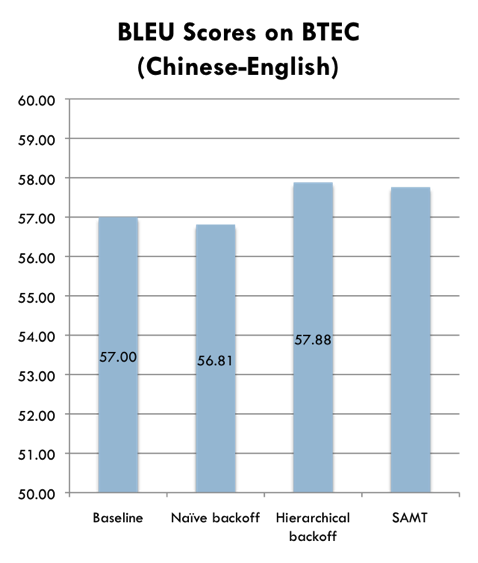
\includegraphics{btec.png}
\end{figure}

\begin{figure}
\label{fig:urdu}
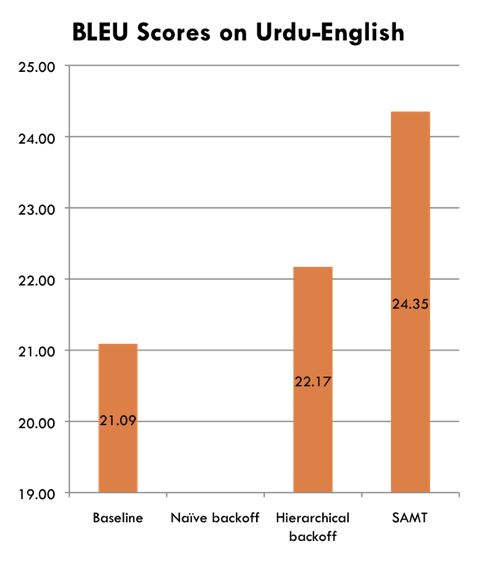
\includegraphics{urdu.png}
\end{figure}

\end{document}